\chapter{Introduction}
\label{cha:introduction}

The work described in this dissertation is concerned with the implementation of a Java solution, named xmlet, that allows the automatic generation of a fluent API based on a XML schema. The generated classes are very similar most of the time and such solution may save time to the user, eliminating repetitive tasks and human error.

\section{Motivation}

%TODO cite

Text has evolved with the advance of technology resulting in the creation of markup languages \cite{markuplanguages}. This markup languages add annotations to text, also known as tags, that allow to add additional information to the text. Each markup language has its own tags and each of those tags add a different meaning to the text encapsulated within them. In order to use markup languages the users can write the text and add all the tags manually, either by fully writing them or by using some kind of text helpers such as intellisense which can help diminish the errors caused by manually writing the tags. But even with text helpers the resulting document can violate the restrictions of the respective markup language. In the following HTML example there is a violation of HTML rules, a <html> tag containing a <div> tag, which isn't allowed.

\newpage

\begin{lstlisting}[caption={Failed HTML rule validation},captionpos=b]
<html>
	<div>
		(...)
	</div>
</html>
\end{lstlisting}

\noindent
The solution to having documents that respect the markup language rules is changing the way the document writing works. If the user has control over the writing process errors can be induced in the document but if the writing control is given to an entity which can enforce the markup languages restrictions then it is guaranteed that the user can't produce a document with errors. In the following code sample the user is allowed to add any child to the Html element, resulting in a violation of the language restrictions, which is only detected during execution.

\begin{lstlisting}[caption={Error validation in runtime},captionpos=b]
	Html root = new Html();
	root.add(new Div());
\end{lstlisting}

In order to create this entity all the restrictions of the given markup language could be recreated in a API and therefore allow the user to generate the document. In the \ref{motivation_2example}, the API enforces the language restrictions in compile time, this way any document generated by this API will be valid.

\begin{figure}[ht]
	\centering
	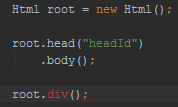
\includegraphics[width=0.4\textwidth]{motivation_2example}
	\caption{Error validation in compile time}
	\label{motivation_2example}
\end{figure}

The only problem with this solution is recreating all the rules of a given markup language, which can be a very long process since most markup languages have a vast number of elements and restrictions. 

\noindent
The solution for this problem is automation. An automated process that converts the definition of elements and restrictions of markups languages in classes that represent those elements and methods that enforce those restrictions. With this automated process the application can generate a fluent API that allow the users to write their texts in a fluent way without errors and respecting the markup language semantics. This is the main objective of this work, creating an infrastructure that reads a markup language definition, in XML Schema Definition, and generates an API that allows the users to write well formed documents.

\section{Use case}

The use case that will be used to test and evaluate the solution will be the HTML5 XML schema. In this case we have multiple elements that share behavior and/or attributes that can be generated automatically. The generated classes allow to create a tree of elements that represent a XML document. This approach is very similar to DOM, the difference being that in this case each API will be specific to a given XSD file, in this case the HTML5 specification. The resulting classes can then be processed in different ways since the Visitor pattern is used. This way each different Visitor implementation can use the generated classes to write HTML documents to a stream, a socket or a file. 

\noindent
The generated HTML5 elements API will then be used in the HtmlFlow API, which is also a fluent Java API that is used to write well formed HTML files. With the Visitor pattern the HtmlFlow will only need to implement its own Visitor to achieve its goal. At the moment the HtmlFlow library only supports a set of the HTML elements which were created manually and the rest of the library interacts with those elements in order to write the HTML files. With the help of the solution which will be developed in this work the HtmlFlow will support the whole HTML syntax. 

\newpage

\section{Document Organization}

This document will be separated in five distinct chapters. The first chapter, this one, introduces the problem that was presented. The second chapter presents existent technology that was used. The third chapter explains in detail the different components of the suggested solution. The fourth chapter approaches the deployment and testing of the suggested solution. The fifth and last chapter of this document contains some final remarks and description of future work.